\chapter{Results and Evaluation}
\label{ch:results}

This chapter evaluates Reddit Sentiment Explorer through a system demonstration, a discussion of sentiment classification quality, and an analysis of system performance considerations. The demonstration follows a complete query lifecycle to illustrate the user experience and the information available at each stage.

\section{System Demonstration}
\label{sec:demonstration}

\begin{sloppypar}
To demonstrate the platform, I walk through a complete query lifecycle for the search term ``Sziget Fesztiv\'{a}l'' across four Hungarian subreddits: r/hungary, r/askhungary, r/budapest, and r/hu. The Sziget Festival is one of Europe's largest music and cultural festivals, held annually on \'{O}budai-sziget in Budapest. It is a recurring subject of discussion on Hungarian Reddit, making it a suitable case study because the topic generates both positive and negative opinions and is discussed almost exclusively in Hungarian.
\end{sloppypar}

\subsection{Dashboard Landing Page}

Figure~\ref{fig:dashboard_hero} shows the dashboard in its initial state. The hero section at the top contains the search input, language and theme controls, and a content language selector set to Hungarian. Below the hero, five tabs organize the workspace: Subreddit Scope, Search And Overview, Sentiment Trends, Subreddit Breakdown, and Matched Content Explorer.

\begin{figure}[H]
    \centering
    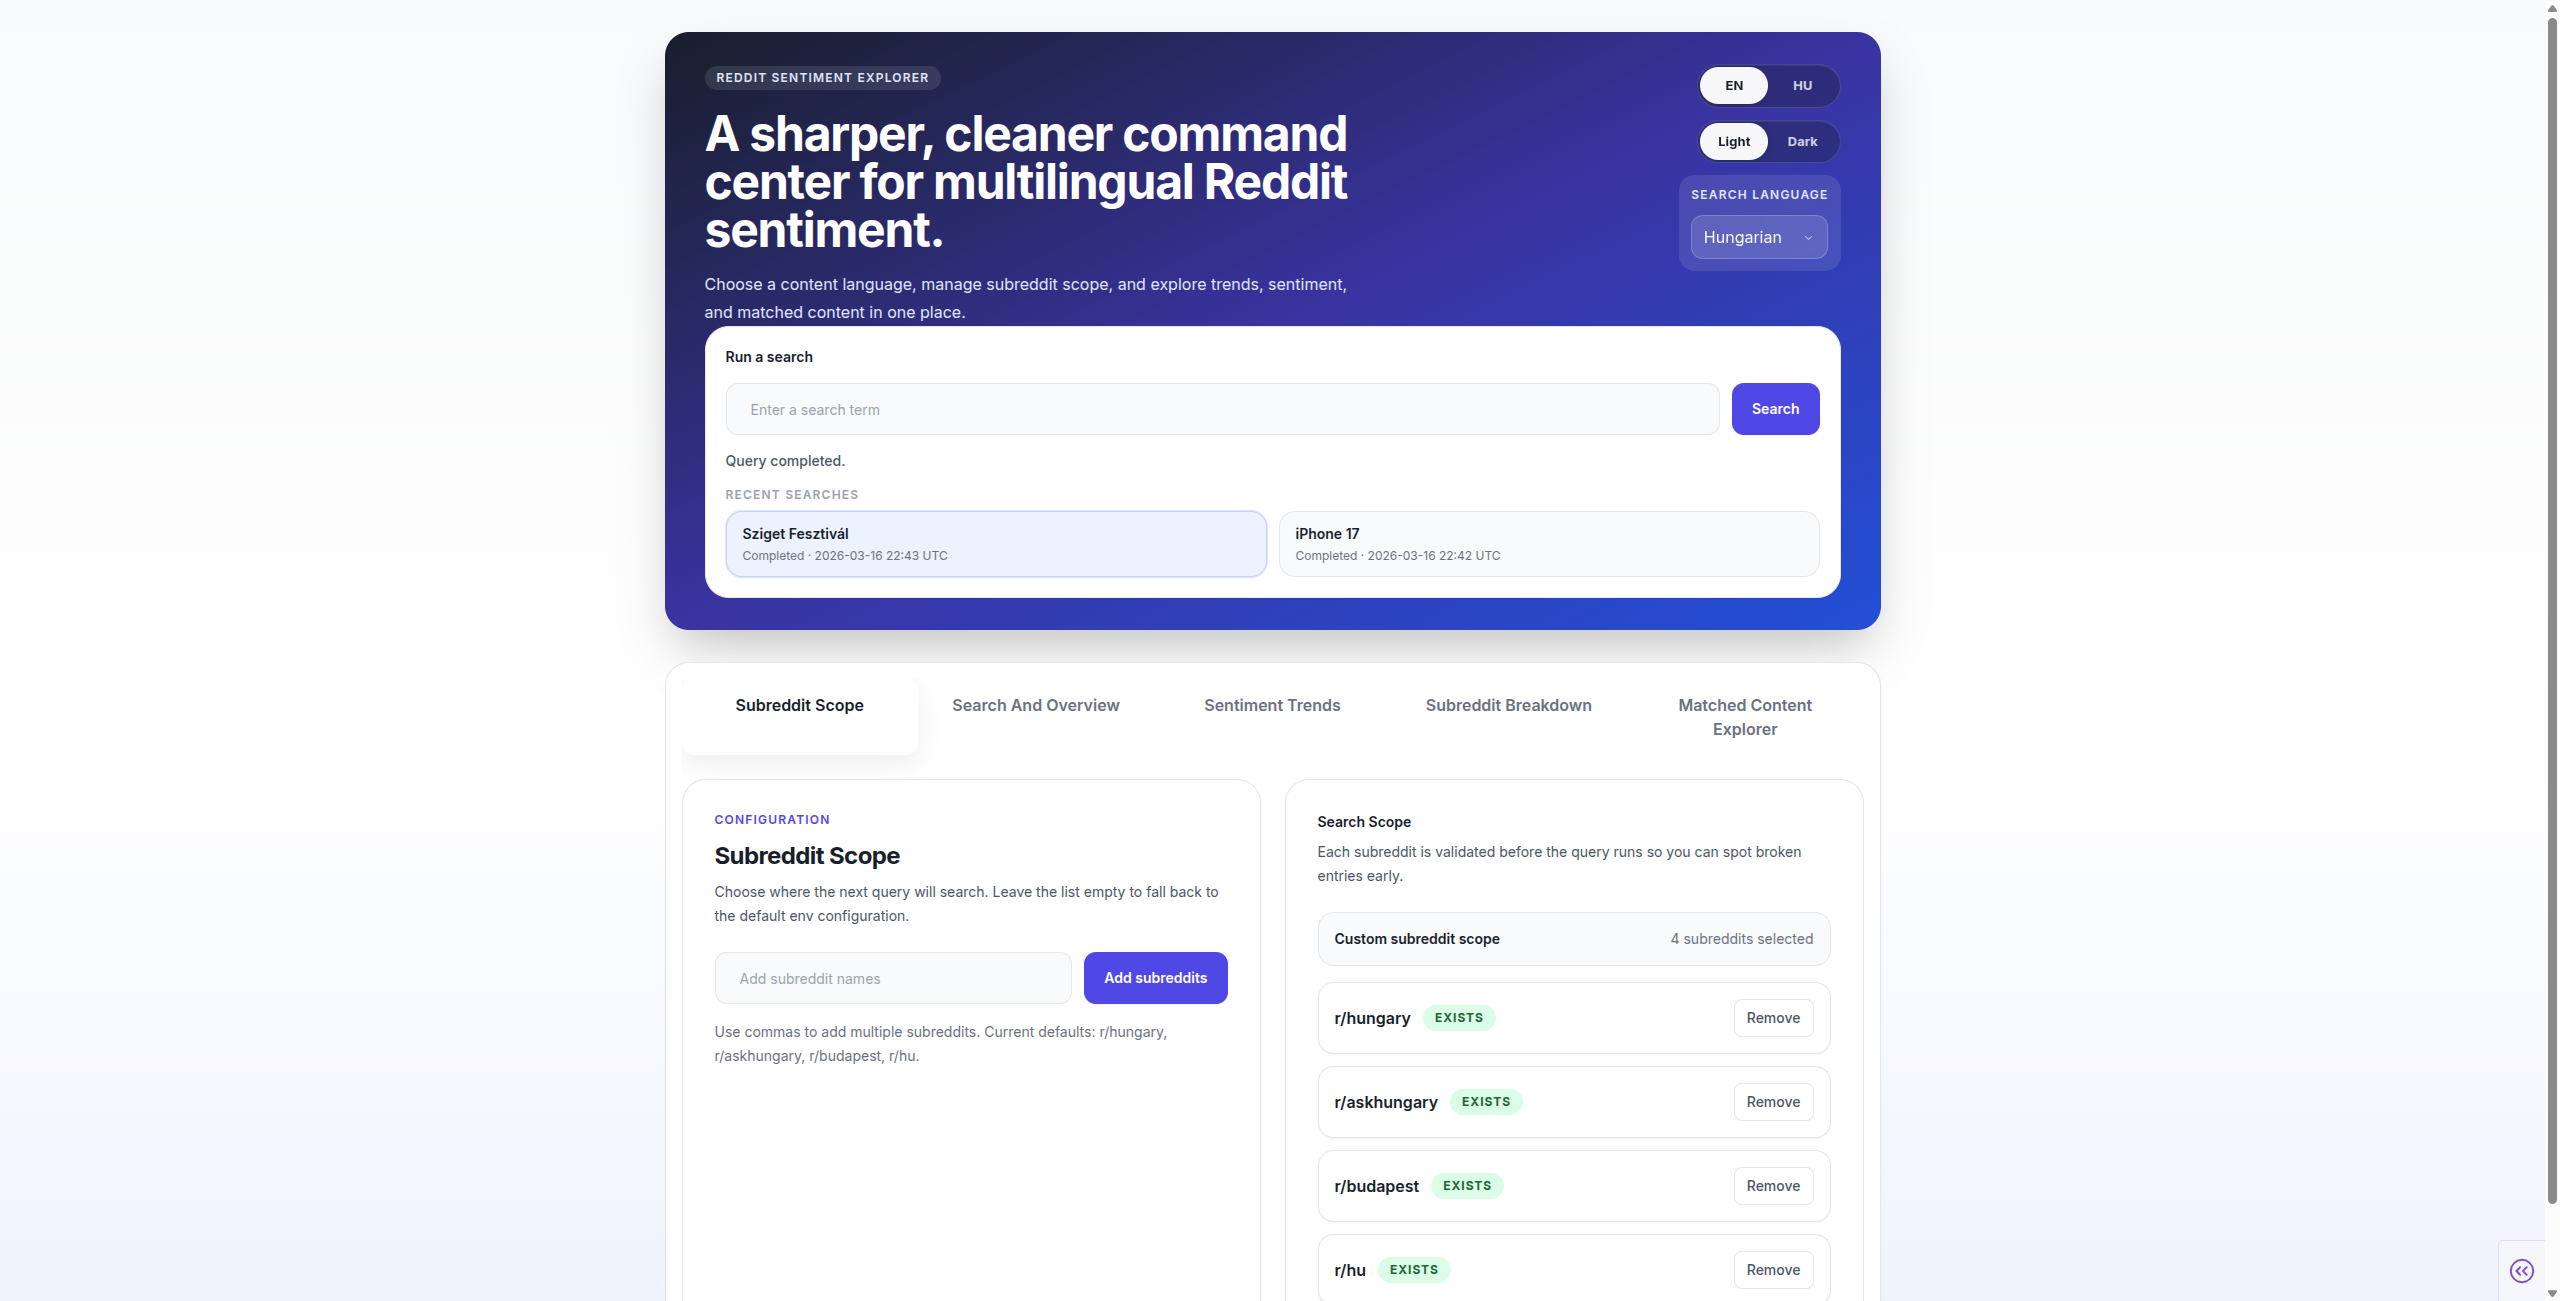
\includegraphics[width=\textwidth]{figures/dashboard-hero.png}
    \caption{Dashboard landing page with search interface and subreddit scope configuration. The left panel allows adding and removing subreddits, while the right panel shows the current scope with validation status.}
    \label{fig:dashboard_hero}
\end{figure}

The Subreddit Scope tab allows users to manage their search scope. Each subreddit is validated against the Reddit API when added, and its status is displayed as a badge. Users can add multiple subreddits at once using comma-separated names.

\subsection{Search Execution}
\label{sec:search_execution}

When the user types ``Sziget Fesztiv\'{a}l'' and clicks Search, the dashboard sends a POST request to the API, which creates a query and a query run. The dashboard then switches to the Search And Overview tab and begins polling the API every five seconds for status updates. A status message indicates that the query is being processed.

The worker picks up the pending run, marks it as running, and begins executing the pipeline: collecting posts and comments from Arctic Shift, matching and filtering content, classifying sentiment via the configured provider, and building aggregates.

\subsection{Search Overview Tab}

Once the pipeline completes, the dashboard displays the results on the Search And Overview tab. This tab provides four main views:

\begin{enumerate}
    \item \textbf{Overview metrics}: a summary card showing the total number of matched documents, the average sentiment score, the number of subreddits searched, and the count of higher- and lower-confidence classifications.
    \item \textbf{Sentiment timeline}: a line chart showing the average sentiment score per day, providing a temporal view of how sentiment evolves over time.
    \item \textbf{Rolling sentiment}: a smoothed seven-day rolling average of the sentiment score, which filters out daily noise and reveals longer-term trends.
    \item \textbf{Sentiment distribution}: a bar chart showing the count of documents in each of the five sentiment categories (very negative through very positive).
\end{enumerate}

Figure~\ref{fig:overview_metrics} shows the Search And Overview tab for the ``Sziget Fesztiv\'{a}l'' query. The overview metrics indicate 171 matched documents with an average sentiment score of $-0.69$, searched across 4 subreddits. The sentiment distribution reveals a predominantly negative skew: 86 documents classified as negative (50.3\%), 39 as neutral (22.8\%), 26 as very negative (15.2\%), and 20 as positive (11.7\%), with no documents classified as very positive. This distribution reflects the contentious nature of recent public discourse around the festival.

\begin{figure}[H]
    \centering
    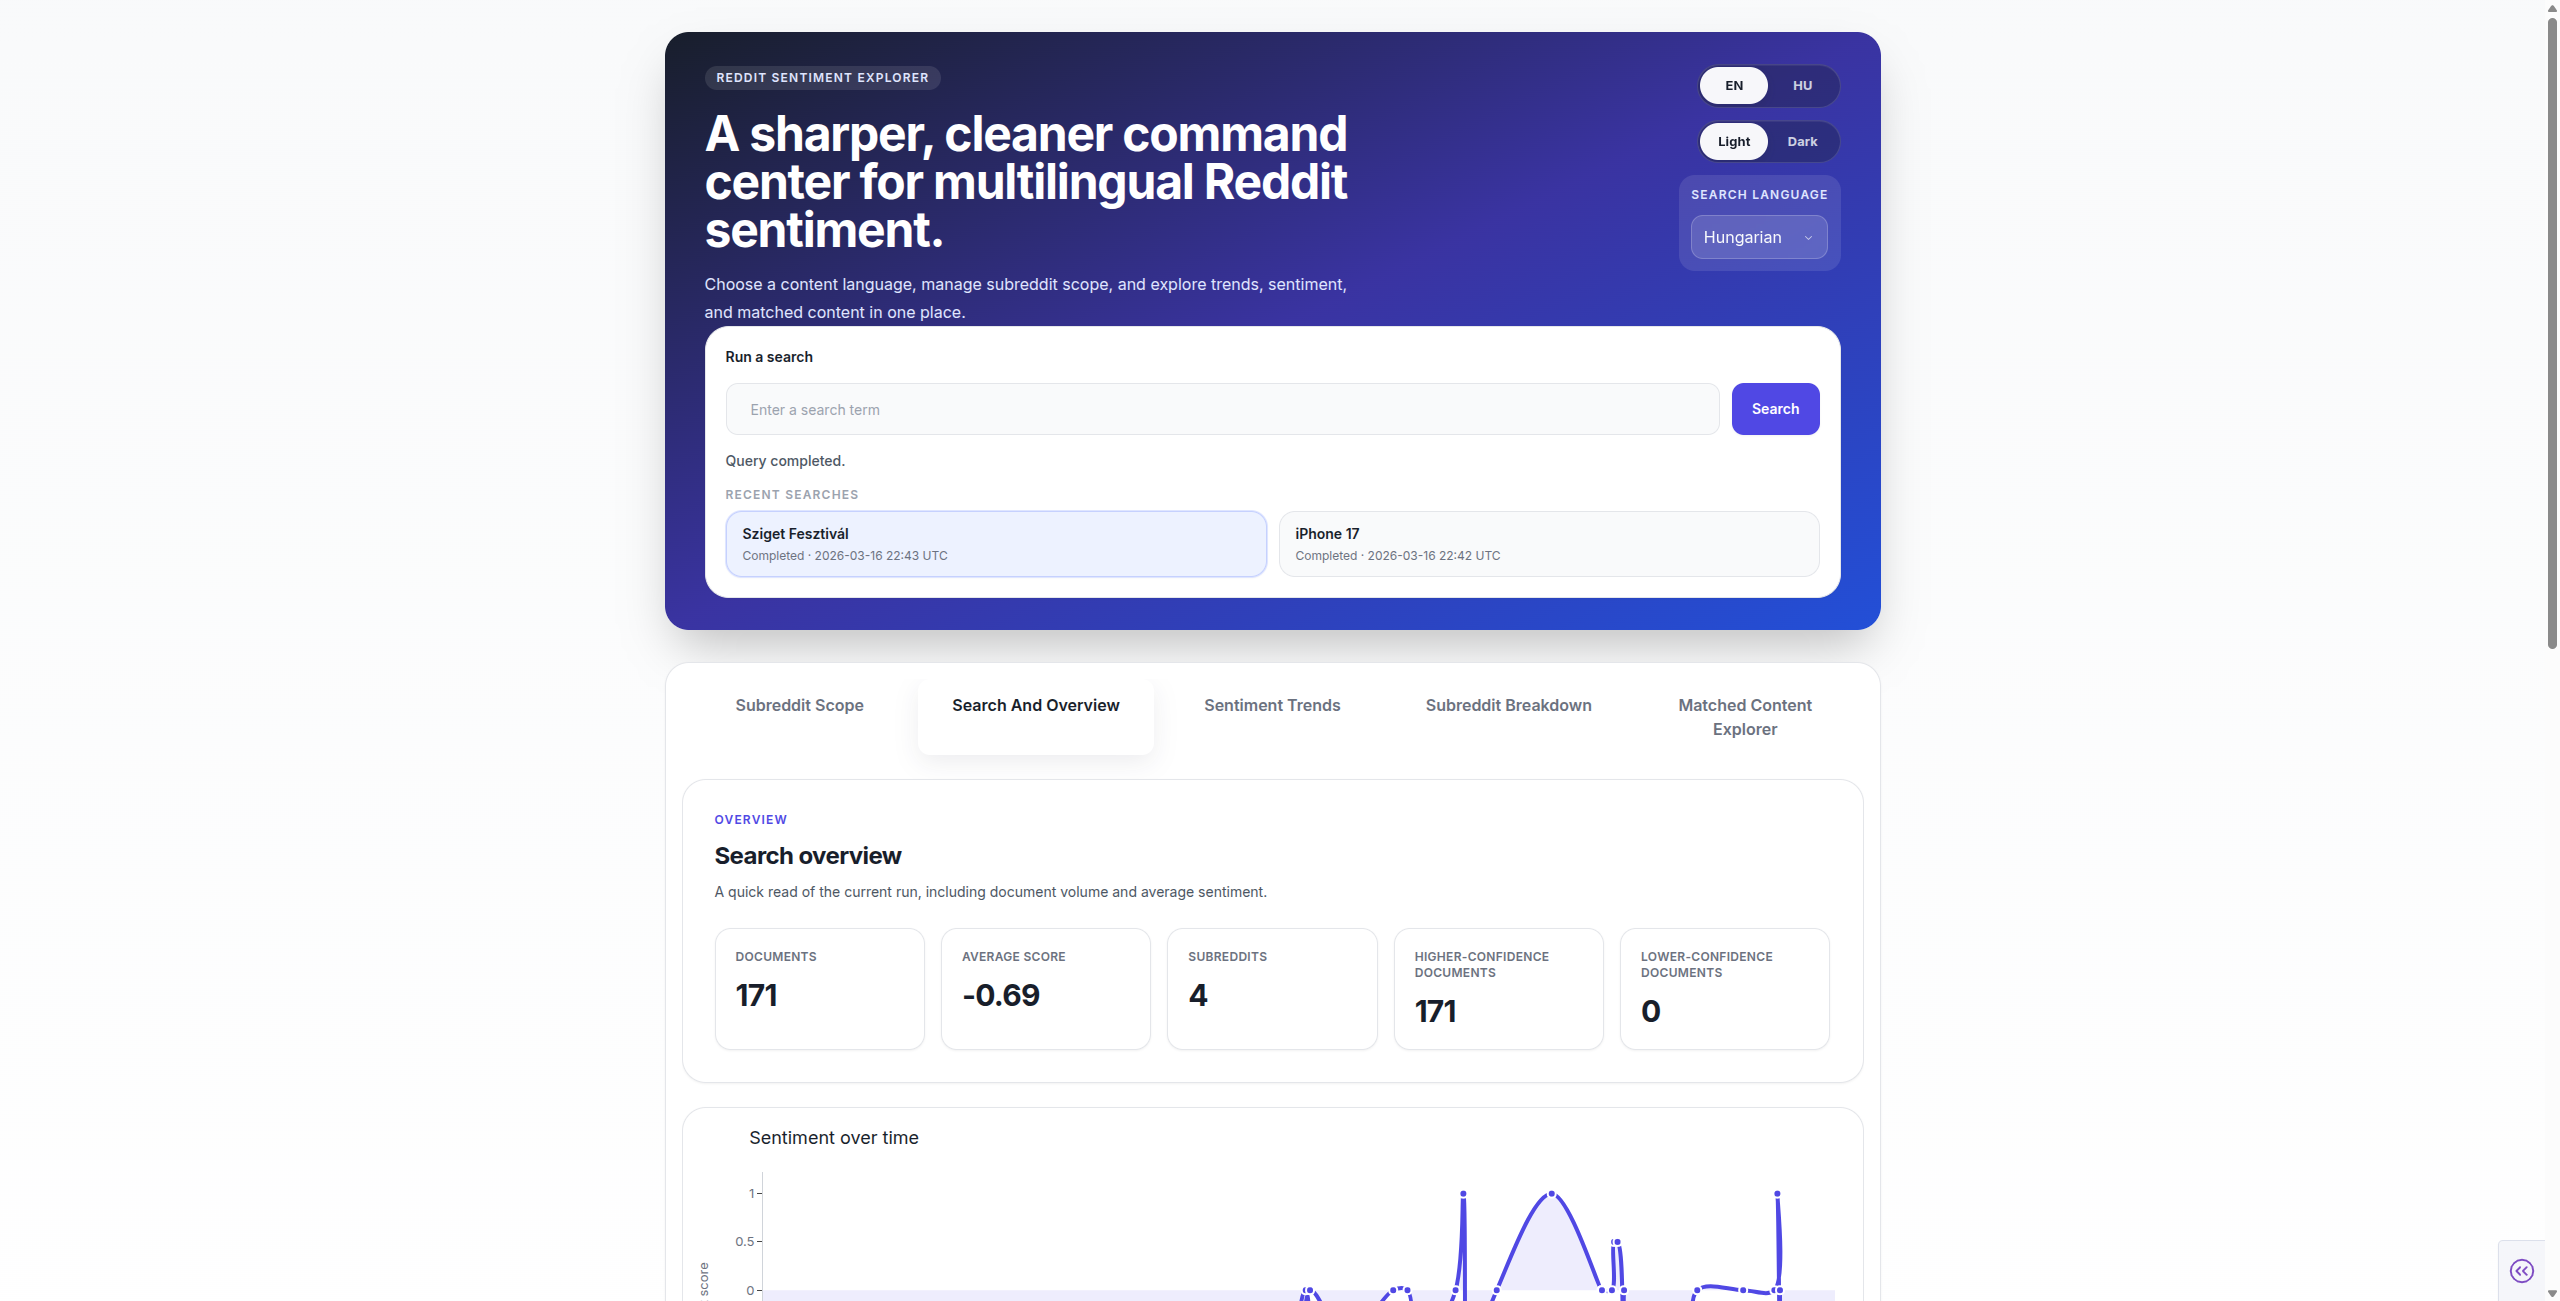
\includegraphics[width=\textwidth]{figures/overview-metrics.png}
    \caption{Search And Overview tab showing overview metrics and the beginning of the sentiment timeline for the ``Sziget Fesztiv\'{a}l'' query across four Hungarian subreddits.}
    \label{fig:overview_metrics}
\end{figure}

These views implement the overview+detail paradigm \cite{cockburn2008overview}. The user immediately sees the high-level picture: how many documents were found, whether overall sentiment is positive or negative, and how it varies over time.

\subsection{Sentiment Trends Tab}

The Sentiment Trends tab provides deeper temporal analysis with three charts:

\begin{enumerate}
    \item \textbf{Sentiment timeline}: same as the overview timeline but displayed at full width for detailed inspection.
    \item \textbf{Volume timeline}: a bar chart showing the number of documents per day, revealing how discussion volume fluctuates.
    \item \textbf{Sentiment heatmap}: a grid showing sentiment scores bucketed by date and subreddit. This reveals which communities discuss the search term and when, for example, showing that r/hungary dominates the conversation while r/askhungary and r/budapest contribute more sporadically.
\end{enumerate}

The content spans from March 2019 to December 2025, with a noticeable spike in discussion volume around late October 2025, when political debates about the festival's future intensified.

\begin{figure}[H]
    \centering
    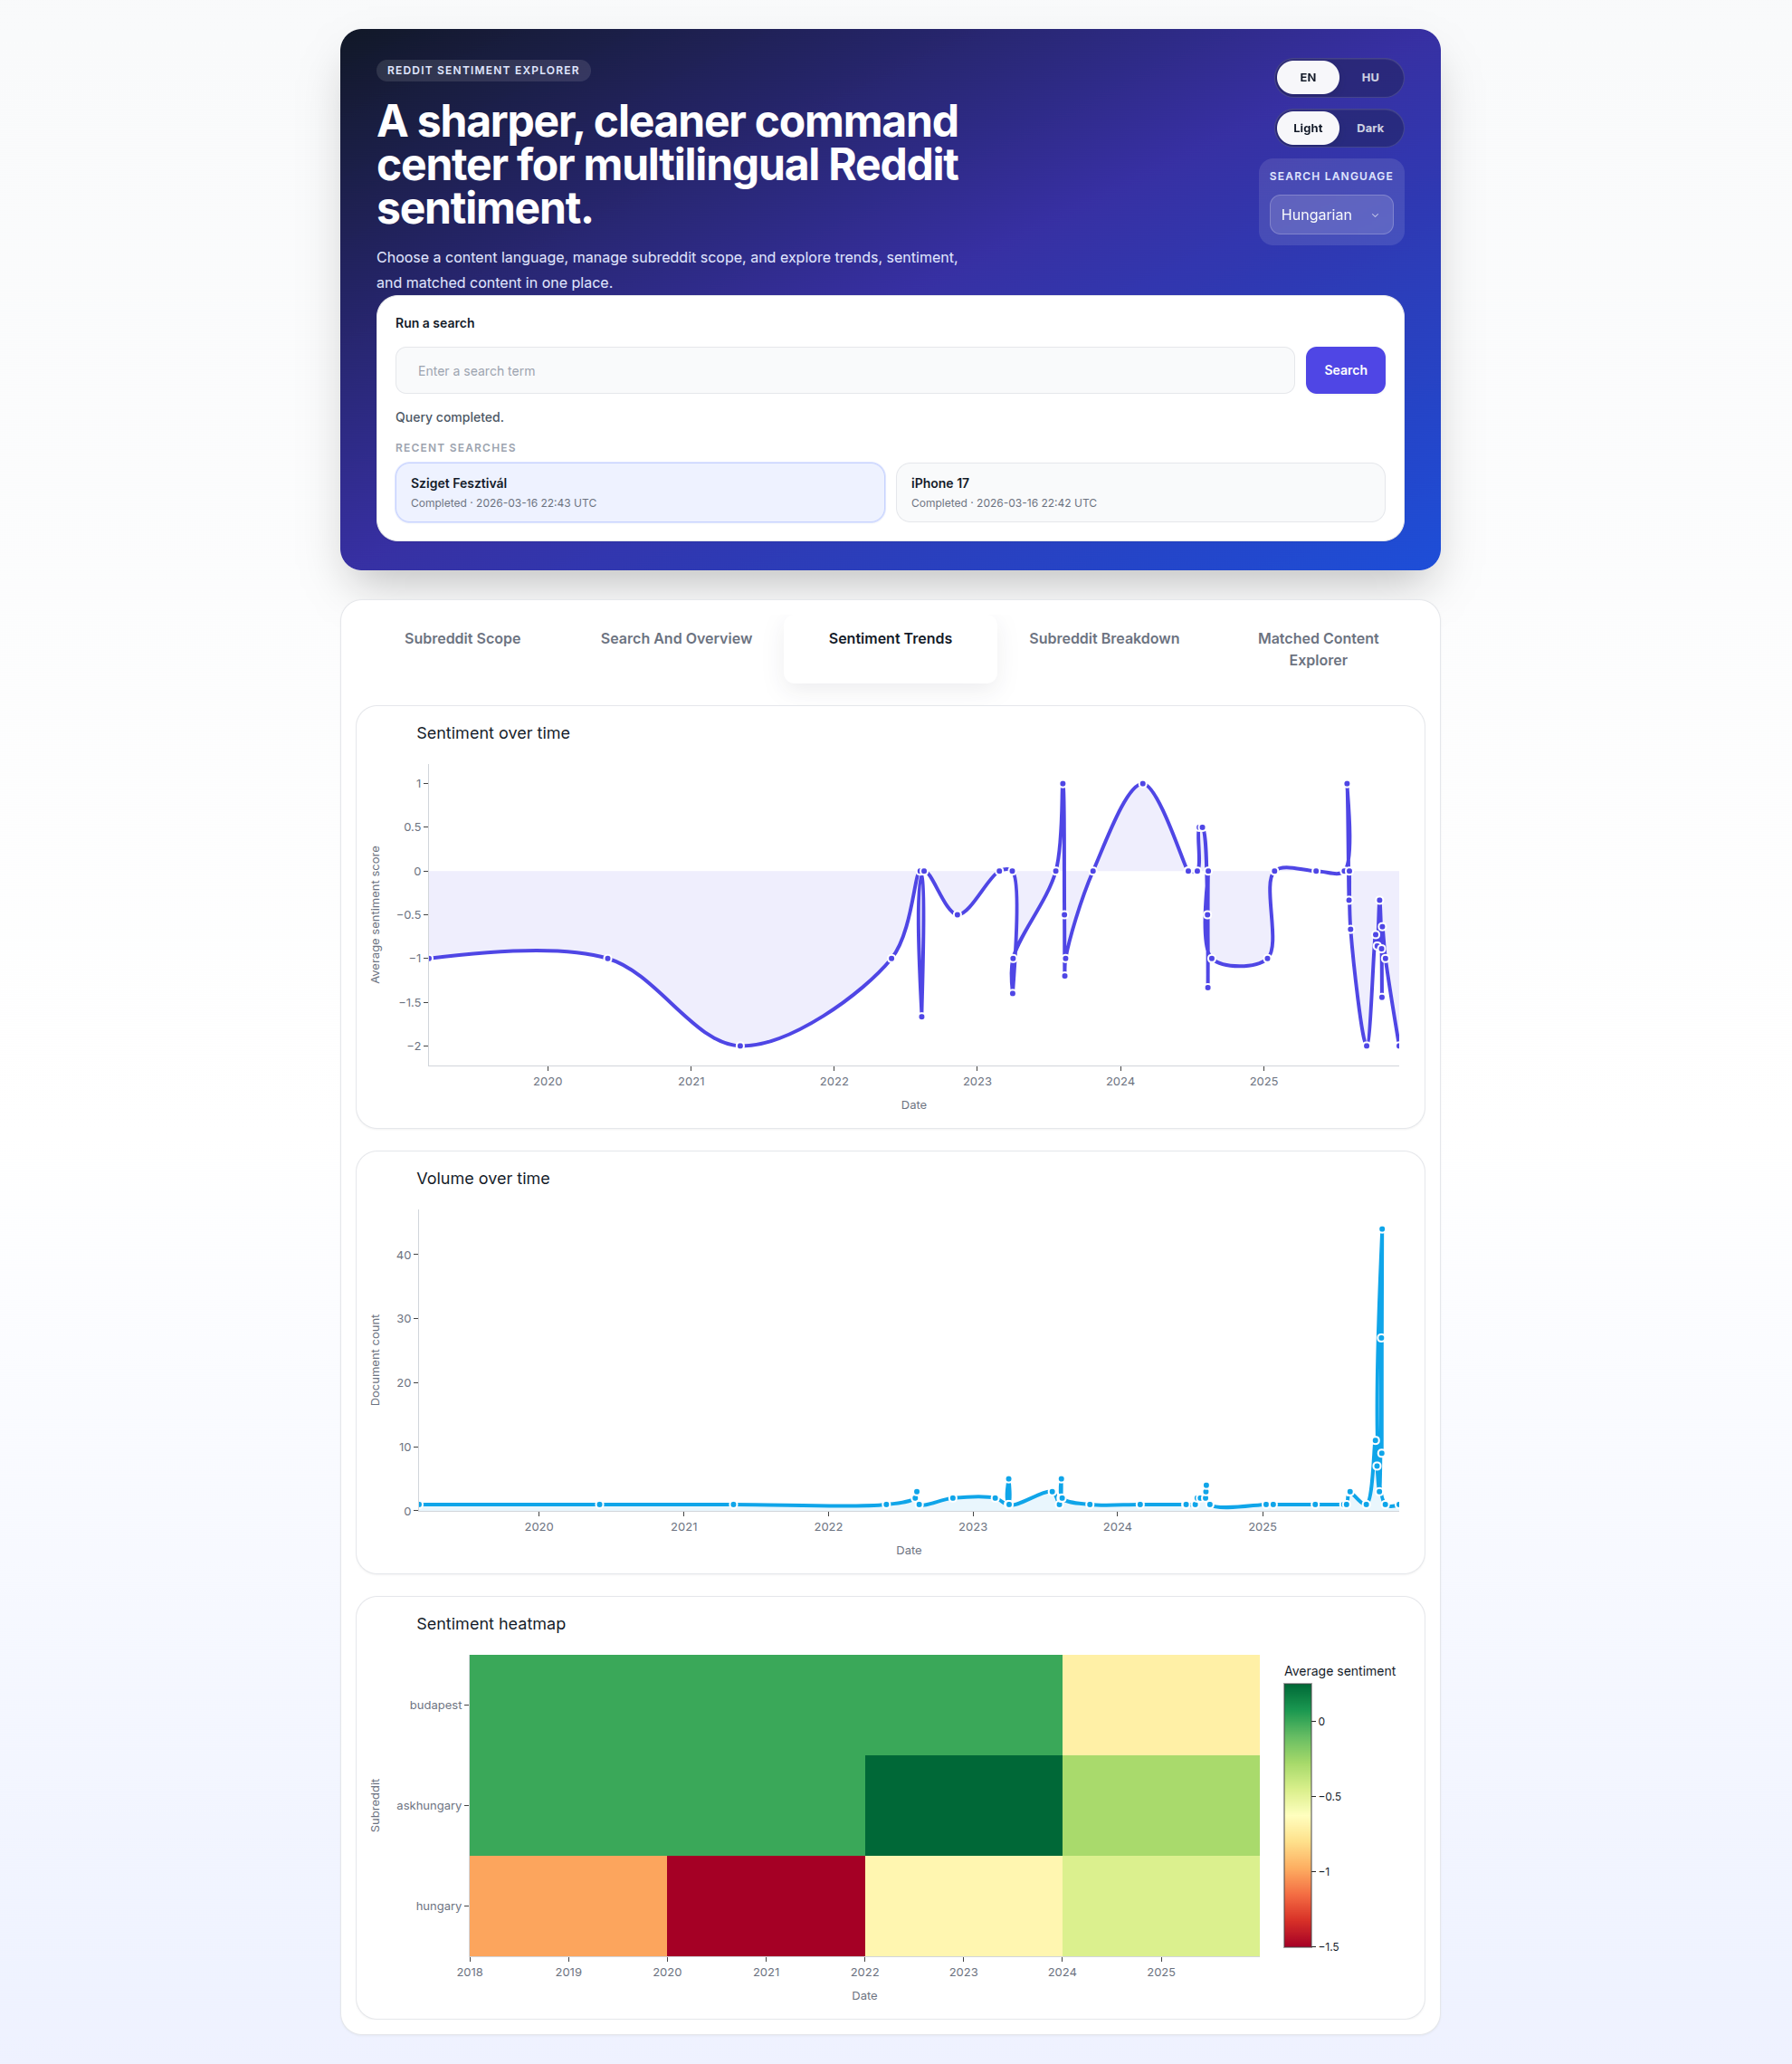
\includegraphics[width=\textwidth]{figures/sentiment-trends.png}
    \caption{Sentiment Trends tab showing the sentiment timeline, volume timeline, and sentiment heatmap for the ``Sziget Fesztiv\'{a}l'' query.}
    \label{fig:sentiment_trends}
\end{figure}

\subsection{Subreddit Breakdown Tab}

The Subreddit Breakdown tab enables comparative analysis across communities:

\begin{enumerate}
    \item \textbf{Subreddit chart}: a stacked bar chart showing the sentiment label distribution for each subreddit. The query returned content from three of the four subreddits: r/hungary (151 documents, average score $-0.75$), r/askhungary (13 documents, average score $0.00$), and r/budapest (7 documents, average score $-0.57$). The r/hu subreddit returned no matching content.
    \item \textbf{Phrase drivers}: evidence phrases grouped by sentiment label, revealing the most common themes. For example, the positive bucket highlights ``j\"{o}v\H{o}re tal\'{a}lkozunk a fesztiv\'{a}lon'' (see you next year at the festival), while the very negative bucket features ``s\'{u}lyos presztizsvesztes\'{e}get'' (serious prestige loss) and ``gyeng\'{\i}ten\'{e} az orsz\'{a}g turisztikai'' (would weaken the country's tourism).
    \item \textbf{Spike events}: a list of dates with unusually high document volume or extreme sentiment, helping users identify specific events that drove discussion.
\end{enumerate}

\begin{figure}[H]
    \centering
    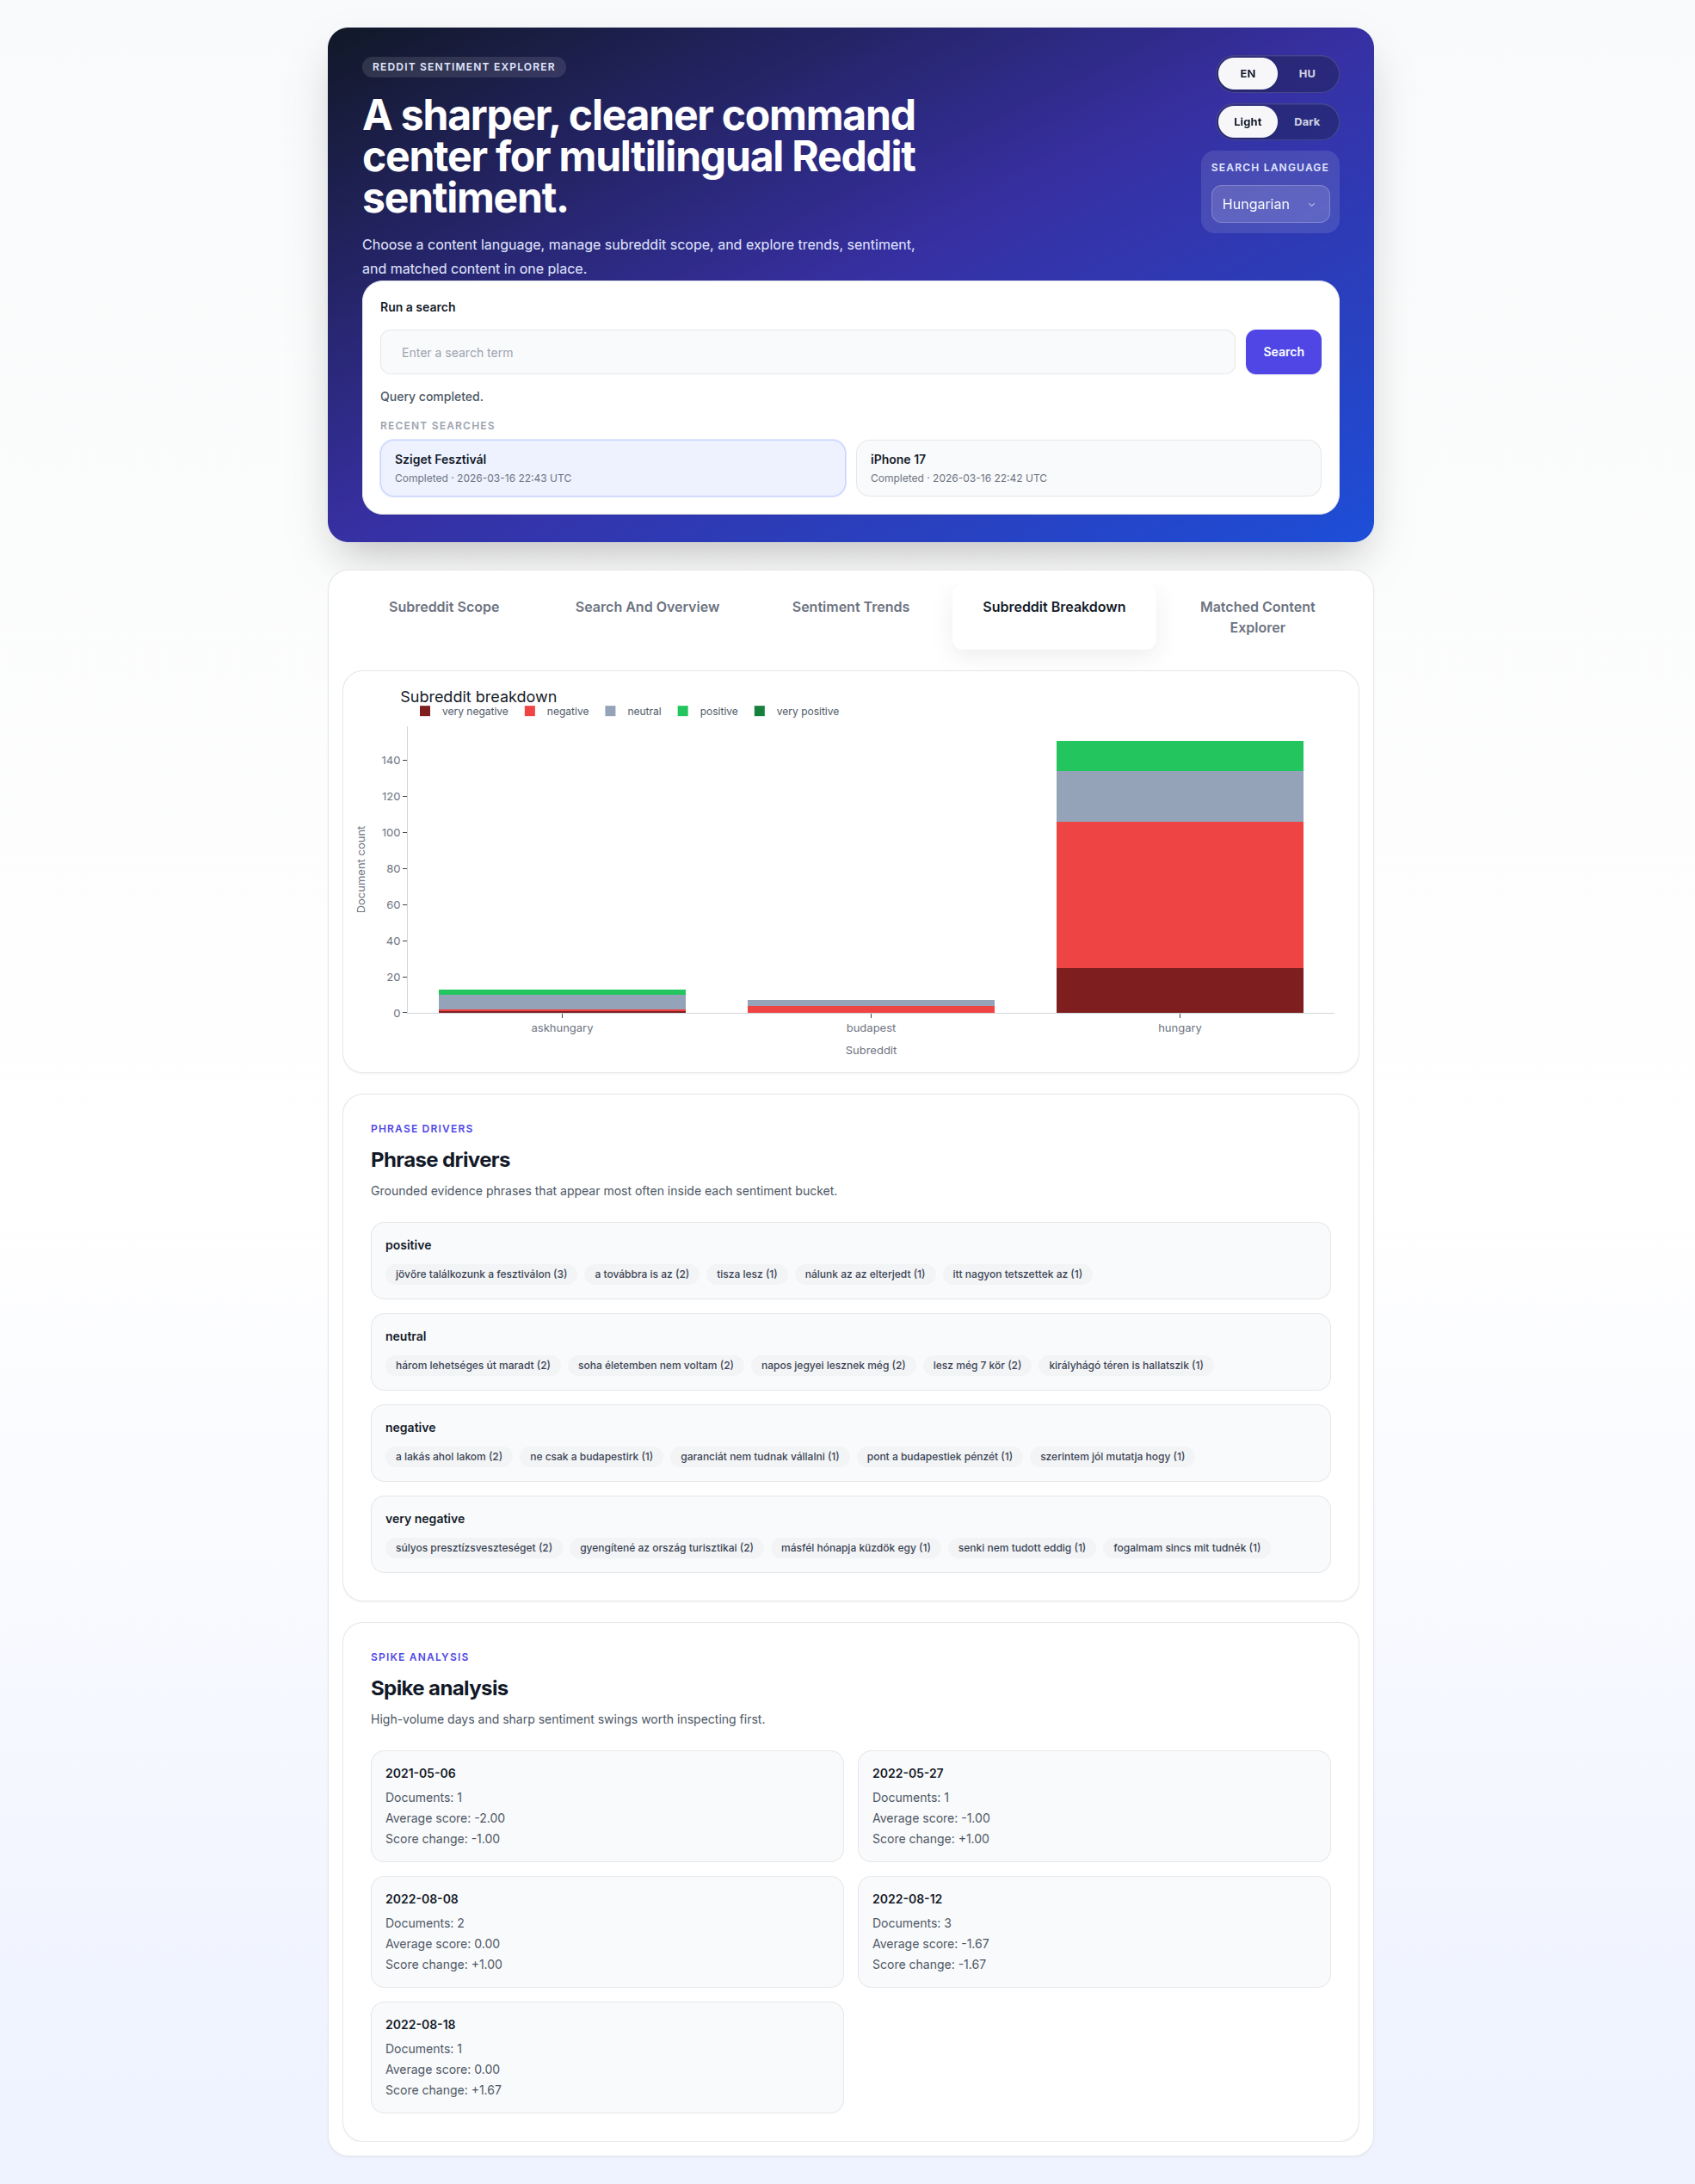
\includegraphics[width=\textwidth]{figures/subreddit-breakdown.png}
    \caption{Subreddit Breakdown tab showing the per-subreddit sentiment distribution, phrase drivers grouped by sentiment label, and spike analysis with notable dates.}
    \label{fig:subreddit_breakdown}
\end{figure}

\subsection{Matched Content Explorer}

The Matched Content Explorer tab provides the ``details on demand'' layer. It lists all matched documents with their sentiment label, source type, date, and a text preview. Users can filter by date, subreddit, sentiment, and source type, or search within the snippet text. Clicking any row expands its full details, including:

\begin{itemize}
    \item The complete text of the post or comment.
    \item The sentiment label and numeric score.
    \item The confidence level of the classification.
    \item The rationale explaining why the model assigned this label.
    \item Evidence phrases: exact quotes from the text that support the classification.
    \item A link to the original Reddit post or comment.
\end{itemize}

Figure~\ref{fig:matched_content} shows the Matched Content Explorer filtered to positive documents, with a selected comment that reads: ``Sosem voltam a Szigeten, mert nem nekem val\'{o} zen\'{e}k vannak ott, de tagadhatatlan, hogy eg\'{e}sz Eur\'{o}p\'{a}ban az egyik legnagyobb zenei fesztiv\'{a}l'' (I've never been to Sziget because the music isn't my style, but it's undeniable that it's one of the largest music festivals in all of Europe). The model classified this as positive with 0.85 confidence, with the rationale noting that the text highlights the festival's positive impact despite the author's personal preferences. The evidence phrases quote passages about the festival being one of the largest in Europe, visitors spending money and enjoying themselves, and Budapest being one of Europe's most beautiful cities.

\begin{figure}[H]
    \centering
    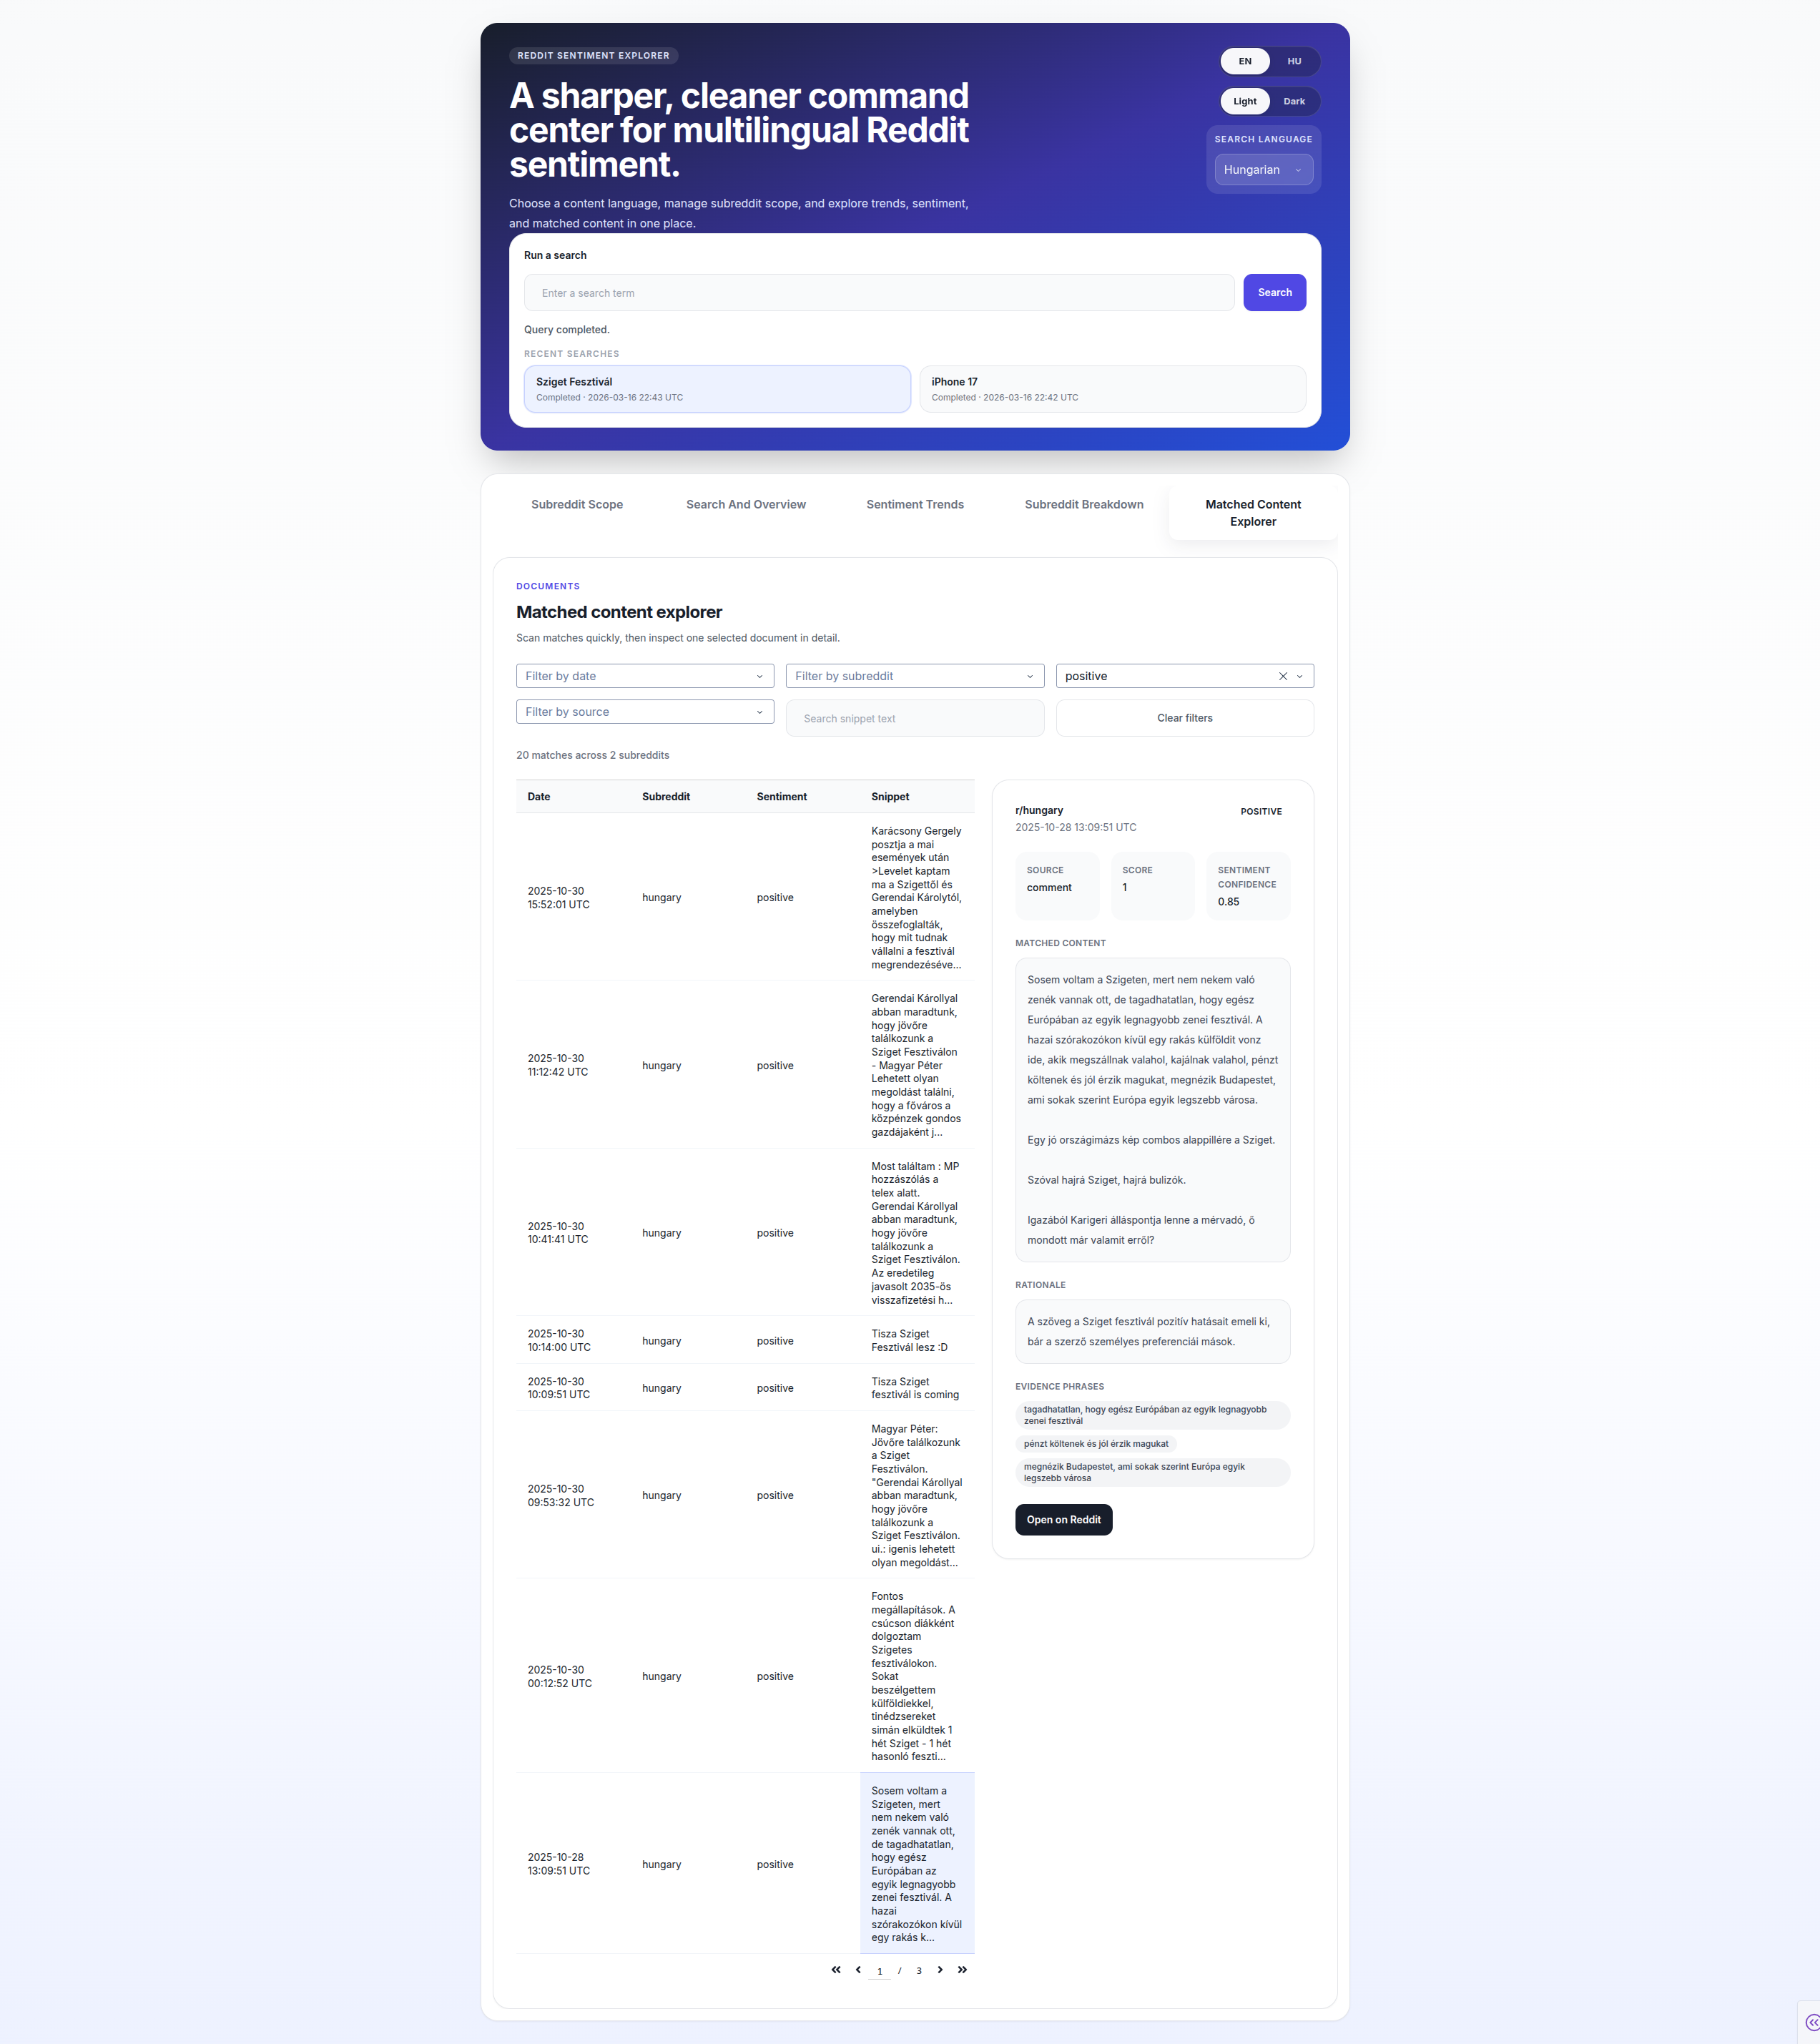
\includegraphics[width=\textwidth]{figures/matched-content.png}
    \caption{Matched Content Explorer filtered to positive documents, showing a comment classified as positive with the rationale in Hungarian and evidence phrases extracted from the source text.}
    \label{fig:matched_content}
\end{figure}

This example demonstrates the model's ability to look beyond surface-level cues: the author explicitly states they have never attended the festival, yet the overall tone is supportive. A keyword-based classifier would struggle to determine sentiment from this text, whereas the LLM correctly identifies the positive framing.

\section{Sentiment Classification Quality}
\label{sec:classification_quality}

I evaluate the sentiment classification quality by examining the outputs of the OpenAI provider and comparing them with the mock provider.

\subsection{OpenAI Provider Strengths}

The OpenAI provider (using GPT-4o-mini) demonstrates several strengths in classifying Reddit content:

\begin{enumerate}
    \item \textbf{Context understanding.} The model understands implicit sentiment, sarcasm, and opinions embedded in longer narratives. For example, a comment that begins with a personal disclaimer (``I've never been there'') but proceeds to praise the festival's economic and cultural value is correctly classified as positive.

    \item \textbf{Multilingual capability.} All 171 documents in this query were detected as Hungarian, and the model classified them without requiring a separate model or translation step. The rationale is provided in Hungarian when the input is Hungarian, making it accessible to the end user.

    \item \textbf{Interpretable output.} The rationale and evidence phrases provide transparency into the classification decision. This is a substantial improvement over traditional classifiers that output only a label and a probability.

    \item \textbf{Fine-grained discrimination.} The model distinguishes between ``negative'' and ``very negative,'' capturing the intensity of sentiment. A comment expressing mild disappointment about ticket prices is classified as negative, while a text describing ``serious prestige loss'' and ``weakening the country's tourism brand'' receives a very negative label with 0.95 confidence.
\end{enumerate}

\subsection{OpenAI Provider Limitations}

\begin{enumerate}
    \item \textbf{Non-determinism.} The same text may receive different labels across runs due to the stochastic nature of language model generation. While the system mitigates this through result caching (the same document is only classified once per provider), different query runs may produce slightly different aggregate statistics for the same content.

    \item \textbf{Cost.} Each classification requires an API call, which incurs a cost. For a query that matches 171 documents, the cumulative cost is noticeable. The current implementation processes documents sequentially, which also contributes to pipeline execution time.

    \item \textbf{Latency.} Each API call takes approximately 0.5--2 seconds, depending on input length and model load. For a query with 171 matched documents, classification alone can take 2--5 minutes.

    \item \textbf{Occasional format errors.} Despite the structured JSON output format, the model occasionally returns confidence as a string (``high'' instead of 0.8) or omits fields. The implementation handles these cases through a confidence normalization method and default values.
\end{enumerate}

\subsection{Comparison with Mock Provider}

The mock provider uses word-counting heuristics and serves as a baseline. It is fast (instant classification) and free (no API costs), but has clear limitations:

\begin{itemize}
    \item It cannot detect sarcasm, irony, or implicit sentiment.
    \item It treats all occurrences of positive/negative words equally regardless of context.
    \item Its word lists are limited and do not cover domain-specific vocabulary.
    \item It assigns fixed confidence values (0.5--0.6) regardless of the actual ambiguity of the text.
\end{itemize}

In informal testing on Hungarian Reddit content, the OpenAI provider produced more nuanced and contextually appropriate results. The mock provider tended to classify most content as neutral due to the limited Hungarian word list, while the OpenAI provider identified a wider range of sentiment intensities.

\section{System Performance}
\label{sec:performance}

\subsection{Pipeline Throughput}

The end-to-end pipeline time depends primarily on two factors: the number of documents collected and the speed of sentiment classification. Data collection from Arctic Shift typically takes 5--15 seconds depending on the number of subreddits and the volume of matching content. Sentiment classification with the OpenAI provider dominates the execution time, processing documents sequentially at 0.5--2 seconds per document.

For the ``Sziget Fesztiv\'{a}l'' query, the pipeline collected 59 posts and 112 comments across three subreddits, classified all 171 matched documents, and built nine types of aggregates. The complete pipeline execution took approximately three minutes.

\subsection{Caching Effectiveness}

The TTL-based caching strategy (default 12 hours) effectively eliminates redundant pipeline executions. Repeated queries for the same term, subreddit scope, and language return cached results instantly. The cache hit rate depends on usage patterns; in a scenario where multiple users explore the same topics, caching provides substantial time and cost savings.

\subsection{Database Performance}

PostgreSQL handles the workload efficiently for the scale of this application. The \texttt{FOR UPDATE SKIP LOCKED} pattern for worker task claiming adds minimal overhead. Precomputed aggregates ensure that chart rendering requires only a single row lookup per aggregate type, regardless of the number of underlying documents.

\section{Discussion}
\label{sec:discussion}

\subsection{Addressing the Research Questions}

\textbf{Research Question 1: How can a modular, query-driven system be designed to collect, filter, and classify Reddit content by sentiment?}

The implementation demonstrates that a four-service architecture with a clear pipeline of stages (collect, persist, match, filter, classify, aggregate) achieves the goal. The separation of concerns enables each component to be developed, tested, and modified independently. The provider abstraction makes sentiment classification pluggable. The Document entity provides a clean abstraction layer between Reddit-specific data and the classification pipeline. The caching strategy and background worker pattern keep the user interface responsive despite long-running classification tasks.

\textbf{Research Question 2: How effectively can large language models classify sentiment in informal, multilingual social media text?}

The ``Sziget Fesztiv\'{a}l'' case study demonstrates that GPT-4o-mini correctly handles Hungarian-language informal text, including political commentary, sarcasm, and nuanced opinions. The model produced interpretable, contextually appropriate classifications across all 171 documents, with high confidence scores (all above the lower-confidence threshold). The rationale and evidence phrases, provided in the language of the source text, add a layer of transparency that traditional classifiers do not offer. The trade-offs (non-determinism, per-call cost, latency) are acceptable for a query-driven exploration tool but would require mitigation for high-volume production use.

\subsection{Comparison with Existing Approaches}

\begin{sloppypar}
Compared to the fragmented scripting approach common in academic research, Reddit Sentiment Explorer provides an integrated, interactive experience from search to visualization. Compared to commercial social listening platforms, it is open-source, customizable, and supports arbitrary search terms without predefined topic constraints. The main limitation relative to commercial tools is scalability: the current single-worker architecture is suited for individual exploration rather than large-scale enterprise monitoring.
\end{sloppypar}
